\chapter{Power Series Method: The Ultimate Guess}
Solution techniques for differential equations lead most to believe that there is a
certain amount of educated guesswork to get started writing a solution.  To some extent
this observation is correct!  Think about the method of undetermined coefficients; built
on an educated guess.  Why don't we just make the ultimate guess: \\
If $y(t)$ is a solution to a differential equation and so long as $y$ is expected to have
a Taylor series representation, then why don't we just guess that $y(t)$ \underline{is} a Taylor
series and use some detective work to determine the coefficients.  To demonstrate this
consider the next problem.

\section{Taylor Series Solutions to Diff. Equations}\label{sec:Taylor_ODE}
In the following problems we are assuming that the solution to the differential equation
can be written in terms of a Taylor series centered at $t=0$
\[ y(t) = \sum_{n=0}^\infty \frac{f^{(n)}(0)}{n!}t^n. \]
\begin{problem}
    Consider the differential equation $y' = y$ with $y(0) = 1$.  
    \begin{enumerate}
        \item[(a)] Solve this differential equation using any appropriate technique.
            \solution{$y(t) = e^t$}
        \item[(b)] Let's assume that $y(t) = \sum_{n=0}^\infty \frac{y^{(n)}(0)}{n!} t^n$ (a Taylor series
            centered at $t=0$).  Expanding the Taylor series we see that
            \[ y(t) = y(0) + y'(0)t + \frac{y''(0)}{2!}t^2 + \frac{y'''(0)}{3!}t^3 +
            \frac{y^{(iv)}(0)}{4!}t^4 + \cdots \]
            From the initial condition we know that $y(0) = 1$ so we at least know that 
            \[ y(t) = 1 + y'(0)t + \frac{y''(0)}{2!}t^2 + \frac{y'''(0)}{3!}t^3 +
            \frac{y^{(iv)}(0)}{4!}t^4 + \cdots \]
            Using the differential equation determine $y'(0)$.
            \solution{$y'(0) = y(0) = 1$ so the Taylor series starts as $y(t) = 1 + t +
            \cdots$}
        \item[(c)] You should now have the first two terms in the Taylor series.
            Differentiate both sides of the differential equation and use your answer to
            determine $y''(0)$.
            \solution{
                Since $y' = y$ we see that $y'' = y'$ so $y''(0) = y'(0) = 1$ and hence
                the Taylor series is now
                \[ y(t) = 1 + t + \frac{1}{2} t^2 + \cdots \]
            }
        \item[(d)] Finally, use what you did in part (c) to determine the rest of the
            Taylor series.  Verify your answer off of part (a).
            \solution{
                \[ y(t) = 1 + t + \frac{t^2}{2} + \frac{t^3}{3!} + \cdots = e^t. \]
            }
    \end{enumerate}
\end{problem}

The previous problem suggests a technique for building the Taylor series of a solution to
a differential equation.  Let's put it into action on another problem that isn't quite as
easy.
\begin{problem}
    Consider the differential equation
    \[ y' - ty = 1 \]
    with initial condition $y(0) = 1$.  
    \begin{enumerate}
        \item[(a)] This problem would traditionally require integrating factors.  Start
            the process of integrating factors and work the procedure until you get to an
            integral that cannot be evaluated.
            \solution{\\
                For integrating factors we let $\rho(t) = e^{\int -t dt} = e^{-t^2/2}$.
                If we multiply both sides of the differential equation by this integrating
                factor and rearrange the left-hand side then
                \[ \frac{d}{dt} \left[ e^{-t^2/2} y  \right] = e^{-t^2/2}. \]
                If we integrate both sides of the differential equation then
                \[ e^{-t^2/2} y = \int e^{-t^2/2} dt. \]
                The right-hand side, however, does not have a known analytic
                antiderivative.  Hence we have to stop here.
            }
        \item[(b)] Now rearrange the differential equation to solve for $y'$ and use that
            rearrangement to determine $y'(0)$, $y''(0)$, $y'''(0)$, etc.
            \solution{
                \begin{flalign*}
                    y(0) &= 1 \\
                    y' &= ty + 1 \\
                    \implies y'(0) &= 0\cdot y(0) + 1 = 1 \\
                    y''(t) &= ty'(t) + y(t) \\
                    \implies y''(0) &= 0 \cdot y'(0) + y(0) = 1 \\
                    y'''(t) &= \left( t y''(t) + y'(t) \right) + y'(t) = ty''(t) + 2y'(t) \\
                    \implies y'''(0) &= 0\cdot 1 + 2 = 2 \\
                    y^{(iv)} &= \left( t y'''(t) + y''(t) \right) + 2y''(t) = ty'''(t) +
                    3y''(t) \\
                    \implies y^{(iv)}(0) &= 0 \cdot 2 + 3 \cdot 1 = 3 \\
                    y^{(v)} &= \left( t y^{(iv)} + y''' \right) + 3y''' = t y^{(iv)} +
                    4y''' \\
                    \implies y^{(v)}(0) &= 0\cdot 3 + 4\cdot 2 = 8 \\
                    y^{(vi)} &= \left( t y^{(v)} + y^{(iv)} \right) + 4y^{(iv)} = ty^{(v)}
                    + 5 y^{(iv)} \\
                    \implies y^{(vi)}(0) &= 0 \cdot 8 + 5 \cdot 3 = 15
                \end{flalign*}
            }
        \item[(c)] Write the Taylor series solution for the differential equation.
            \solution{
                \[ y(t) = 1 + t + \frac{1}{2}t^2 + \frac{2}{3!} t^3 +
                    \frac{3}{4!} t^4 + \frac{8}{5!} + t^5 + \cdots \]
            }
        \item[(d)] Use a plotting tool to create a plot of the approximate Taylor series
            solution using the first several terms in the Taylor series.
            \solution{
                \begin{center}
                    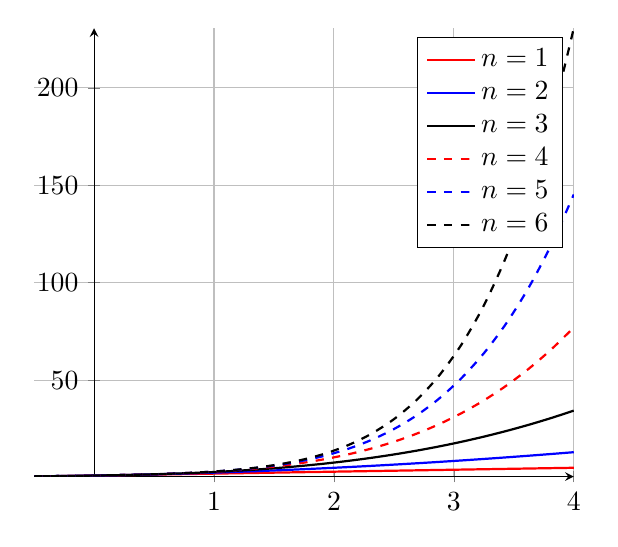
\begin{tikzpicture}
                        \begin{axis}[axis lines=center, grid]
                            \addplot[smooth, thick, red, domain=-0.5:4] {1+x};
                            \addlegendentry{$n=1$};
                            \addplot[smooth, thick, blue, domain=-0.5:4] {1+x+0.5*x^2};
                            \addlegendentry{$n=2$};
                            \addplot[smooth, thick, black, domain=-0.5:4] {1+x+0.5*x^2 +
                            (1/3)*x^3};
                            \addlegendentry{$n=3$};
                            \addplot[smooth, thick, red, dashed, domain=-0.5:4] {1+x+0.5*x^2 +
                            (1/3)*x^3+(1/6)*x^4};
                            \addlegendentry{$n=4$};
                            \addplot[smooth, thick, blue, dashed, domain=-0.5:4] {1+x+0.5*x^2 +
                            (1/3)*x^3+(1/6)*x^4 + (1/15)*x^5};
                            \addlegendentry{$n=5$};
                            \addplot[smooth, thick, black, dashed, domain=-0.5:4] {1+x+0.5*x^2 +
                            (1/3)*x^3+(1/6)*x^4 + (1/15)*x^5+ (15/720)*x^6};
                            \addlegendentry{$n=6$};
                        \end{axis}
                    \end{tikzpicture}
                \end{center}

            }
    \end{enumerate}
\end{problem}

\begin{problem}
    Summarize the technique of using Taylor series to approximate the solution to a
    differential equation.
\end{problem}

\begin{problem}
    Use the Taylor series method to estimate a solution to the differential equation
    \[ y'' - 2ty' + 2y = 0 \]
    with $y(0) = 1$ and $y'(0)=-1$.
\end{problem}
\solution{
    Since $y(0) =1 $ and $y'(0) = -1$ the Taylor series starts as 
    \[ y(t) = 1 - t + \cdots.\]
    Since $y'' - 2ty + 2y = 0$ we can rewrite to get $y'' = 2ty' - 2y$.  Hence $y''(0) =
    2(0)(-1) - 2(1) = -2.$  Therefore,
    \[ y(t) = 1 - t - \frac{2}{2!} t^2 + \cdots.\]
    Next, $y'''(t) = 2ty'' + 2y' - 2y' = 2ty''$ so $y'''(0) = 2(0)(-2) = 0$.  Therefore,
    \[ y(t) = 1 - t - t^2 + 0t^3 + \cdots. \]
    For the next step, $y^{(iv)} = 2ty''' + 2y''$ so $y^{(iv)}(0) = 2(0)(0) + 2(-2) = 4$
    so
    \[ y(t) = 1 - t - t^2 + 0t^3 + \frac{4}{4!} t^4 + \cdots \]
    \begin{center}
        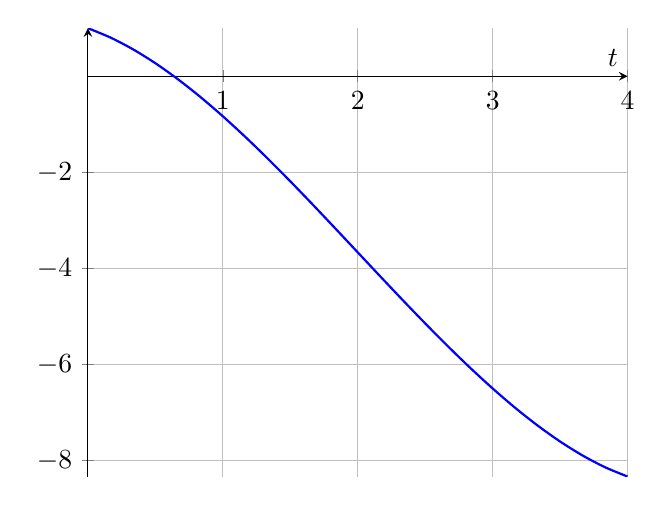
\begin{tikzpicture}
            \begin{axis}[axis lines=center, xlabel={$t$}, grid]
                \addplot[smooth, blue, thick, domain=0:4] {1 - x - x^2 + (1/6)*x^3};
            \end{axis}
        \end{tikzpicture}
    \end{center}
}



\section{Radius of Convergence for Power Series (INCOMPLETE)}
A power series is an infinite series of power functions
\[ y(t) = \sum_{n=0}^\infty a_n t^n. \]
We observe that the Taylor series discussed previously is just a special kind of power
series, but that is not the only kind that is interesting.  Power series, in general, can
be used to build up functions that cannot be written in terms of regular algebraic or
trigonometric functions.  The ``infinity'' in the upper bound on the sum, however, could
cause some problems.  It is not generally true to say that any power series will create a
new function.  For poor choices of the coefficients $a_n$ the sum may diverge to infinity
for all values of $t$.  What we need is an arsenal of tools to determine whether or not a
power series actually converges to something meaningful or if it diverges off to infinity.
The primary tools are summarized in the following problems and theorems.


\begin{problem}
    We start this investigation just looking at sums of numbers.  Write computer code to
    determine the sums
    \begin{flalign*}
        &\sum_{n=0}^{5} \frac{n!}{2^n} = \underline{\hspace{1in}}\\
        &\sum_{n=0}^{50} \frac{n!}{2^n} = \underline{\hspace{1in}}\\
        &\sum_{n=0}^{500} \frac{n!}{2^n} = \underline{\hspace{1in}}\\
        &\sum_{n=0}^{5000} \frac{n!}{2^n} = \underline{\hspace{1in}}
    \end{flalign*}
    and now make a conjecture: Does the series 
    \[ \sum_{n=0}^\infty \frac{n!}{2^n} \]
    converge to a finite value or diverge to infinity?
\end{problem}
\solution{
This clearly diverges}

\begin{problem}
    Now let's consider a more interesting series that maybe isn't so obvious.
    Write computer code to determine the sums
    \begin{flalign*}
        &\sum_{n=0}^{5} \frac{n^2}{(2n-1)!} = \underline{\hspace{1in}}\\
        &\sum_{n=0}^{50} \frac{n^2}{(2n-1)!} = \underline{\hspace{1in}}\\
        &\sum_{n=0}^{500} \frac{n^2}{(2n-1)!} = \underline{\hspace{1in}}\\
        &\sum_{n=0}^{5000} \frac{n^2}{(2n-1)!} = \underline{\hspace{1in}}
    \end{flalign*}
    and now make a conjecture: Does the series 
    \[ \sum_{n=0}^\infty \frac{n^2}{(2n-1)!} \]
    converge to a finite value or diverge to infinity?
\end{problem}
\solution{
    This series converges.
}

\begin{problem}
    Each of the previous two problems were written in the form $\sum_{n=0}^\infty a_n$
    where $a_n$ is the sequence of numbers being summed.  
    \begin{enumerate}
        \item For the sum 
            \[ \sum_{n=0}^\infty \frac{n!}{2^n} \]
            determine $a_n$ and find the limit
            \[ \lim_{n\to\infty} \left| \frac{a_{n+1}}{a_n} \right|. \]\solution{The limit
            is infinite}
        \item For the sum 
            \[ \sum_{n=0}^\infty \frac{n^2}{(2n-1)!} \]
            determine $a_n$ and find the limit
            \[ \lim_{n\to\infty} \left| \frac{a_{n+1}}{a_n} \right|. \]\solution{The limit
            is zero}
    \end{enumerate}
\end{problem}

\begin{problem}
    Consider the series
    \[ \sum_{n=0}^\infty \frac{n^2 + 2n +1 }{3^n + 2}. \]
    Write computer code that finds sums for successivaly larger and larger upper bounds.
    Use this computer code to conjecture whether this series converges or diverges.
    Finally, evaluate the limit
    \[ \lim\left| \frac{a_{n+1}}{a_n} \right| \]
    where $a_n = \frac{n^2 + 2n + 1}{3^n + 2}$.
\end{problem}
\solution{The series converges and the limit is $1/3$.
}


The {\it ratio test} that follows is a test to determine if a series will converge or
diverge.  
\begin{thm}[The Ratio Test]
    Let $a_n$ be a sequence of numbers and consider the sum $\sum_{n=0}^\infty a_n$.  
    \begin{itemize}
        \item If $\ds \lim_{n\to\infty} \left| \frac{a_{n+1}}{a_n} \right| < 1$ then the
            sum converges to a finite value.
        \item If $\ds \lim_{n\to\infty} \left| \frac{a_{n+1}}{a_n} \right| > 1$ then the
            sum diverges to infinity.
        \item If $\ds \lim_{n\to\infty} \left| \frac{a_{n+1}}{a_n} \right| = 1$ then the
            sum may either converge or diverge.
    \end{itemize}
\end{thm}


\begin{problem}
    Use the ratio test to determine whether the following series converge or diverge.
    \begin{flalign*}
        & \sum_{n=0}^\infty \frac{2^n + 5}{3^n} \\
        & \sum_{n=0}^\infty \frac{1}{n!} \\
        & \sum_{n=1}^\infty \frac{n^n}{n!} \\
        & \sum_{n=1}^\infty \frac{7^{n+2}}{2n6^n} \\
    \end{flalign*}
\end{problem}


Now we switch back to our study of power series.  It is not generally true that we can
just build a power series and we get a meaningful result.  There might only be a small
region where the series converges.  Consider the next problem.
\begin{problem}\label{prob:power_series_conv}
    Consider the power series
    \[ f(x) = 1 - x^2 + x^4 - x^6 + x^8 - x^{10} + \cdots = \sum_{n=0}^\infty
        (-1)^{n} x^{2n} \]
    \begin{enumerate}
        \item[(a)] Write computer code that plots a sequence of functions 
            \[ 1, \quad 1-x^2, \quad 1-x^2 + x^4, \quad 1-x^2+x^4-x^6, \quad \ldots. \]
            Based on your sequence of plots where does the power series converge?
            \solution{
            \begin{center}
                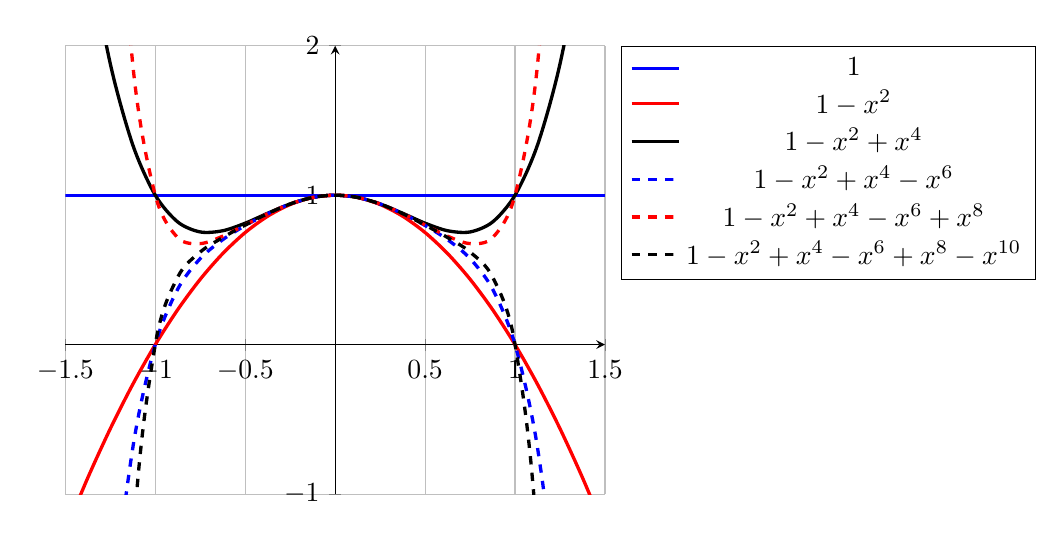
\begin{tikzpicture}
                    \begin{axis}[axis lines=center, domain=-1.5:1.5, xmin=-1.5, xmax=1.5,
                        ymin=-1, ymax=2, grid, legend pos=outer north east]
                        \addplot[smooth, very thick, blue] {1+0*x};
                        \addlegendentry{$1$};
                        \addplot[smooth, very thick, red] {1-x^2};
                        \addlegendentry{$1-x^2$};
                        \addplot[smooth, very thick, black] {1-x^2+x^4};
                        \addlegendentry{$1-x^2+x^4$};
                        \addplot[smooth, very thick, blue, dashed] {1-x^2+x^4-x^6};
                        \addlegendentry{$1-x^2+x^4-x^6$};
                        \addplot[smooth, very thick, red, dashed] {1-x^2+x^4-x^6+x^8};
                        \addlegendentry{$1-x^2+x^4-x^6+x^8$};
                        \addplot[smooth, very thick, black, dashed]
                        {1-x^2+x^4-x^6+x^8-x^10};
                        \addlegendentry{$1-x^2+x^4-x^6+x^8-x^{10}$};
                    \end{axis}
                \end{tikzpicture}
            \end{center}
            It seems like the series is converging in $-1 < x < 1$.
        }
        \item[(b)] Let $a_n = (-1)^{n} x^{2n}$ and evaluate the limit 
            \[ \lim \left| \frac{a_{n+1}}{a_n} \right|. \]
            \solution{This limit evaluates to $|x|$}
        \item[(c)] Based on your knowledge of the ratio test, for what values of $x$ does
            the series $\sum_{n=0}^\infty (-1)^{n} x^{2n}$ converge? \solution{This
            series only converges for $|x|<1$}
    \end{enumerate}
\end{problem}

\begin{problem}
    Repeat problem \ref{prob:power_series_conv} with the series
    \[ \sum_{n=0}^\infty \frac{1}{n!} x^n. \]
    Back up any conjectures that you make from the plots with the use of the ratio test.
\end{problem}
\solution{
    This is the Taylor series for $e^x$ and the series converges for all $x\in\mathbb{R}$.
}

\begin{problem}
    Repeat problem \ref{prob:power_series_conv} with the series
    \[ \sum_{n=0}^\infty \frac{(-1)^n n}{4^n} (x+3)^n. \]
    Back up any conjectures that you make from the plots with the use of the ratio test.
\end{problem}
\solution{
    This series converges on $-7 < x < 1$.
}



\begin{thm}[Radius of Convergence of Power Series]
    Given a power series $\sum a_n t^n$ and the limit
    \[ R(x) = \lim_{n \to \infty} \left| \frac{c_{n+1}x^{n+1}}{c_{n}x^n} \right| \]
    exists then
    \begin{itemize}
        \item for all $x$ such that $R(x) < 1$ the power series converges,
        \item for all $x$ such that $R(x) > 1$ the power series diverges.
    \end{itemize}
\end{thm}


\section{Power Series Solutions to Diff. Equations}
Using Taylor series as we did in Section \ref{sec:Taylor_ODE} is one technique for finding
a series solution to differential equations.  In this section we will look at a more
general technique: using power series to build solutions.  This technique streamlines the
Taylor series technique and actually involves must less work for some problems.  
Instead of
saying that $y(t)$ is a Taylor series, $y(t) = \sum_{n=0}^\infty \frac{y^{(n)}}{n!} t^n$
we simply start by saying that $y(t)$ is just a power series with an unknown sequences of
coefficients: 
\[ y(t) = \sum_{n=0}^\infty a_n t^n. \]  
Our detective work from this assumption amounts to massaging the power series and the
differential equation to determine a pattern for the sequence $a_n$.

In order to use power series to build solutions to differential equations we need to be
able to differentiate (and integrate) power series in a meaningful way.  Thankfully, we
are blessed with the following theorem from mathematical analysis.
\begin{thm}\label{thm:series_term_by_term}
    Let $a_n$ be a sequence of real numbers such that the series $\sum_{n=0}^\infty a_n
    x^n$ converges for $x \in (-R,R)$.  The number $R$ is called the radius of convergence
    for the power series.  
    \begin{enumerate}
        \item If $f(x) = \sum_{n=0}^\infty a_n x^n$ then $f'(x) = \sum_{n=1}^\infty n a_n
            x^{n-1}$
        \item If $f(x) = \sum_{n=0}^\infty a_n x^n$ then $f''(x) = \sum_{n=2}^\infty
            n(n-1) a_n x^{n-2}$
        \item If  $f(x) = \sum_{n=0}^\infty a_n x^n$ then $f^{(k)}(x) = \sum_{n=k}^\infty
            n(n-1)\cdots(n-k+1) a_n x^{n-k}$
        \item If $f(x) = \sum_{n=0}^\infty a_n x^n$ then $\int f(x) dx = \sum_{n=0}^\infty
            \frac{a_n}{n+1} x^{n+1}+C$
    \end{enumerate}
\end{thm}
\begin{proof}
    Really, the full proof of this theorem is beyond the scope of this text.  Instead,
    convince yourself that this theorem is true for finite sums (this should be obvious)
    and trust the author that it holds within the radius of convergence for infinite sums.
\end{proof}

Really, Theorem \ref{thm:series_term_by_term} says that so long as you are within the
radius of convergence of the power series then the series can be differentiated or
integrated term by term.  This has an impact on the use of power series for approximating
solutions to differential equations.  We simply assume that we are within the radius of
convergence and proceed with determining the sequence $a_n$ that defines the power series.
Let's look at an example.

\begin{example}
    Consider the differential equation $y' = -0.5y$ with $y(0) = 1$ and assume that $y(t) =
    \sum_{n=0}^\infty a_n t^n$.  Find the sequence $a_n$ that defines the power series.
    \\{\bf Solution:} This is a simple differential equation and we know that solution is $y(t) =
    e^{-0.5t}$.  Let's build the power series.\\
    Assume that $y(t) = \sum_{n=0}^\infty a_n t^n$ so we see that since $y' = -0.5 y$,
    \[ \sum_{n=1}^\infty n a_n t^{n-1} = -\frac{1}{2} \sum_{n=0}^\infty a_n t^n. \]
    Expanding both sides of the summation and then matching terms we get
    \begin{flalign*}
        & 1 a_1 + 2 a_2 t^1 + 3 a_3 t^2 + 4 a_4 t^3 + 5 a_5 t^4 + \cdots =
        -\frac{1}{2} \left( a_0 + a_1 t^1 + a_2 t^2 + a_3 t^3 + a_4 t^4 + a_5 t^5 + \cdots
        \right) \\
        & \implies 0 = \left( -\frac{1}{2} a_0 - a_1 \right) + \left(
        -\frac{1}{2} a_1 - 2 a_2 \right) t + \left( -\frac{1}{2} a_2 - 3a_3 \right) t^2 +
        \left( -\frac{1}{2} a_3 - 4 a_4 \right) t^3 + \cdots \\
        & \implies a_1 = -\frac{1}{2} a_0, \quad a_2 = -\frac{1}{4} a_1 =
        \frac{1}{8} a_0, \quad a_3 = -\frac{1}{6} a_2 = -\frac{1}{48} a_0, \quad a_4 =
        -\frac{1}{8} a_3 = \frac{1}{384} a_0, \quad \ldots
    \end{flalign*}
    Since $y(0) = 1$ we know that $a_0 = 1$ so
    \[ a_0=1, \quad a_1 = -\frac{1}{2}, \quad a_2 = \frac{1}{8}, \quad a_3 =
        -\frac{1}{48}, \quad a_4 = \frac{1}{384}, \quad \ldots \]
    We conclude by writing the Taylor series approximation
    \[ y(t) = 1 - \frac{1}{2} t + \frac{1}{8} t^2 - \frac{1}{48} t^3 +
        \frac{1}{384} t^4 + \cdots. \]
    We can observe that this Taylor series can be rewritten as
    \[ y(t) = 1 + \left( -\frac{t}{2} \right) + \frac{1}{2!} \left( -\frac{t}{2} \right)^2
        + \frac{1}{3!} \left( -\frac{t}{2} \right)^3 + \frac{1}{4!} \left(
        -\frac{t}{2}
        \right)^4 + \cdots = e^{-0.5 t}  \]
    hence recognizing the analytic solution that we knew from separation of variables.
\end{example}

\begin{problem}
    Assume that $y$ is represented as a power series $y(t) = \sum_{n=0}^\infty a_n t^n$
    and find the coefficients $a_n$ for the solution to the differential equation $y' - ty = 1$ with $y(0)
    = 1$.
\end{problem}
\solution{
    Assuming that $y$ is a power series we get
    \[ \sum_{n=1}^\infty \left( n a_n t^{n-1} \right)  - t \sum_{n=0}^\infty \left( a_n t^n
        \right) = 1. \]
    Expanding the left-hand side we get
    \begin{flalign*}
        & \left( a_1 + 2 a_2 t + 3 a_3 t^2 + 4 a_4 t^3 + 5 a_5 t^4 + \cdots \right) - \left(
        a_0 t + a_1 t^2 + a_2 t^3 + a_3 t^4 + a_4 t^5 + \cdots \right) = 1 \\
        &\implies a_1 + (-a_0 + 2a_2) t + (-a_1 + 3a_3) t^2 + (-a_2 + 4a_4) t^3 + (-a_3 +
        5a_5) t^4 + \cdots = 1 \\
        &\implies a_1 = 1, \quad 2a_2 = a_0, \quad 3a_3 = a_1, \quad 4a_4 =
        a_2, \quad \cdots, (k+2)a_{k+2} = a_k \\
        &\implies a_{k+2} = \frac{a_k}{k+2}
    \end{flalign*}
    From the initial condition we know that $a_0 = 1$ so 
    \begin{flalign*}
        a_0 = a_1 = 1 \\
        a_2 = \frac{1}{2}, \quad
        a_3 = \frac{1}{3}, \quad
        a_4 = \frac{1}{8}, \quad
        a_5 = \frac{1}{15}, \quad
        a_6 = \frac{1}{48}, \quad \cdots
    \end{flalign*}
    and the power series solution is
    \[ y(t) = 1 + t + \frac{1}{2} t^2 + \frac{1}{3} t^3 + \frac{1}{8} t^4 +
        \frac{1}{15} t^5 + \frac{1}{48} t^6 + \cdots. \]
}

\begin{problem}
    Assume that $y$ is represented as a power series $y(t) = \sum_{n=0}^\infty a_n t^n$
    and find the coefficients $a_n$ for the solution to the differential equation
    \[ t^2 y'' + ty' + t^2 y = 0 \quad \text{with} \quad y(0) = 1. \]
    This function is called a {\bf Bessel function of the first kind} and shows up in the
    study of wave phenomenon.  Use a graphing utility (and enough terms in the series) to
    show a plot of $y(t)$ on the domain $t \in [0,6]$.
\end{problem}
\solution{
    We assume that $y(t)$ can be written as a power series and expand each term on the
    left-hand side of teh differential equation.
    \begin{flalign*}
        t^2 y'' &=  t^2 \sum_{n=2}^\infty n(n-1) a_n t^{n-2}\\ 
        &= t^2 \left( (2)(1) a_2 + (3)(2) a_3 t + (4)(3) a_4 t^2 + \cdots + (k)(k-1) a_k
        t^{k-2} + \cdots \right)\\
        &= (2)(1) a_2 t^2 + (3)(2) a_3 t^3 + (4)(3) a_4 t^4 + (5)(4) a_5 t^5 + \cdots +
        (k)(k-1) a_k t^k + \cdots \\ 
        ty'&= t \sum_{n=1}^\infty n a_n t^{n-1} \\
        &= t \left( 1 a_1 + 2 a_2 t + 3 a_3 t^2 + 4 a_4 t^3 + 5 a_5 t^4 + \cdots + k a_k
        t^{k-1} \right) \\
        &= a_1 t + 2 a_2 t^2 + 3 a_3 t^3 + 4 a_4 t^4 + 5 a_5 t^5 + \cdots + k a_k t^k +
        \cdots \\
        t^2y &= t^2 \sum_{n=0}^\infty a_n t^{n} \\
        &= a_0 t^2 + a_1 t^3 + a_2 t^4 + a_3 t^5 + a_4 t^6 + \cdots + a_{k-2} t^{k} + \cdots 
    \end{flalign*}
    Adding these three terms we see that the $k^{th}$ power of $t$ has coefficient
    $(k)(k-1) a_k + (k) a_k + a_{k-2}$ and the fact that the right-hand side of the
    differential equation is zero implies that $k^2 a_k = -a_{k-2}$.  Hence the
    coeeficients in the power series are
    \[ a_k = \frac{-a_{k-2}}{k^2}. \]
    Hence the coefficients of the power series are
    \[ a_0 = 1, \quad a_1 = 0, \quad a_2 = -\frac{a_0}{2^2} = -\frac{1}{4}, \quad a_3 =
        -\frac{a_1}{3^2} = 0, \quad a_4 = -\frac{a_2}{4^2} = \frac{a_0}{2^2 4^2} =
        \frac{1}{2^2 4^2} 
        \]
        \[ a_5 = -\frac{a_3}{5^2} = 0, \quad a_6 = -\frac{a_4}{6^2} =
            -\frac{a_0}{2^2 4^2 6^2} = -\frac{1}{2^2 4^2 6^2}, \quad \cdots \]
    It is clear that each odd indexed coefficient will be zero ($a_1 = a_3 = a_5 = a_7 =
    \cdots = 0$) and for each even index
    \[ a_{2k} = \frac{(-1)^k}{(2k)^2 (2k-2)^2 (2k-4)^2 \cdots 2^2} \]
    \begin{center}
        \begin{tikzpicture}
            \begin{axis}[axis lines=center, domain=0:7, xmin=0, xmax=7];
                \addplot[smooth, very thick, blue, samples=100] {1 - 0.25*x^2 + (1/(4*16))*x^4 -
                (1/(4*16*36))*x^6 + (1/(4*16*36*64))*x^8 - (1/(4*16*36*64*100))*x^(10) +
            (1/(4*16*36*64*100*144))*x^(12) -(1/(4*16*36*64*100*144*196))*x^(14) };
            \end{axis}
        \end{tikzpicture}
    \end{center}
}

\begin{problem}
    Write computer code to generate the plot of the Bessel function in the previous
    problem up to any amount of accuracy.
\end{problem}


\begin{problem}
    Use power series to solve the equation $y'' + ty = 0$ with $y(0) = 1$ and $y'(0) =1$.
    This differential equation gives rise to a function called
    the {\bf Airy equation}.  We saw it as the solution to one of the lab problems at
    the beginning of the semester.
\end{problem}
\solution{
    \begin{flalign*}
        y'' &= \sum_{n=2}^\infty n(n-1)a_n t^{n-2} = (2)(1) a_2 + (3)(2) a_3 t + (4)(3)
        a_4 t^2 + (5)(4) a_5 t^3 + \cdots \\
        ty &= \sum_{n=0}^\infty a_n t^{n+1} = a_0 t + a_1 t^2 + a_2 t^3 + a_3 t^4 +
        \cdots.
    \end{flalign*}
    From here we see that 
    \[ 0 = 2 a_2 + \left( (3)(2) a_3 + a_0 \right) t + \left( (4)(3) a_4 + a_1 \right) t^2
    + \left( (5)(4) a_5 + a_2 \right) t^3 + \cdots \left( (k)(k-1) a_k + a_{k-3} \right)
t^{k-2} + \cdots \]
    From the initial conditions we know that $a_0 = a_1= 1$.  From the previous equation we also
    know that $a_2 = 0$.  Generally, 
    \[ a_k = \frac{-a_{k-3}}{k(k-1)} \quad \text{for} \quad k\ge 3. \]
    Therefore,
    \[ a_0=1, \quad a_1 = 1, \quad a_2 = 0, \quad a_3 = -\frac{a_0}{(3)(2)} =
    -\frac{1}{(3)(2)}, \quad a_4 = -\frac{a_1}{(4)(3)} = -\frac{1}{(4)(3)}, \ldots \]
}

\begin{problem}
    Find the first four terms in the power series expansion of the solution to the
    differential equation
    \[ \left( t^2 + 1 \right) y'' - 4t y' + 6y = 0 \quad \text{with} \quad y(0) = y'(0) =
        1. \]
\end{problem}
\solution{
    Assuming that $y(t) = \sum_{n=0}^\infty a_n t^n$ we get the following solution.
    From the initial conditions we know that $a_0 = a_1 = 1$.
    We'll start breaking the differential equation apart term by term.  
    \begin{flalign*}
        \left( t^2 + 1 \right) y'' &= \left(t^2 + 1 \right) \left( (2)(1) a_2 + (3)(2) a_3
        t + (4)(3) a_4 t^2 + (5)(4) a_5 t^3 + \cdots \right) \\
        &= \left( (2)(1) a_2 t^2 + (3)(2) a_3 t^3 + (4)(3) a_4 t^4 + (5)(4) a_5 t^5 +
        \cdots \right) \\
        & \quad + \left( (2)(1) a_2 + (3)(2) a_3 t + (4)(3) a_4 t^2 + (5)(4) a_5 t^3 +
        \cdots \right) \\
        -4t y' &= (-4t) \left( (1)a_1 + (2) a_2 t + (3) a_3 t^2 + (4) a_4 t^3 + \cdots
        \right) \\
        &= -4 a_1 t - (4)(2) a_2 t^2 - (4)(3) a_3 t^3 - (4)(4) a_4 t^4 + \cdots \\
        &= -4t - (4)(2) a_2 t^2 - (4)(3) a_3 t^3 - (4)(4) a_4 t^4 + \cdots \\
        -6y &= -6 a_0 - 6 a_1 t - 6 a_2 t^2 - 6 a_3 t^3 - 6 a_4 t^4 - 6 a_5 t^5 - \cdots\\
        &= -6 - 6 t - 6a_2 t^2 - 6 a_3 t^3 - 6 a_4 t^4 - 6 a_5 t^5 - \cdots
    \end{flalign*}
    Gathering like terms in the differential equation we see that
    \begin{flalign*}
        0 &= \left( -6 + 2a_2 \right) + \left( -6 -4 + 6 a_3 \right) t + \left( -6a_2 -
        8a_2 + 12 a_4 + 2a_2 \right) t^2 + \cdots
    \end{flalign*}
    which implies that $a_2 = 3$, $a_3 = \frac{5}{3}$, and $a_4 = 3$.  Therefore
    \[ y(t) \approx 1 + t + 3t^2 + \frac{5}{3} t^3 + 3t^4 + \cdots . \]
}
